%! Author = hilfiker
%! Date = 21.07.2022

% Preamble
\documentclass[11pt]{article}

% Packages
\usepackage{amsmath} % Formulas in document
\usepackage{pdflscape} % Landscaped pages in Pdf
\usepackage[a4paper, margin=0.8in]{geometry} % Set the margin and size of a page
\usepackage[hidelinks]{hyperref} % Remove Boxes around Hyperlinks
\usepackage{lastpage} % Custom page numbering
\usepackage{pgfgantt} % Gantt-Tables
\usepackage{fancyhdr}
\usepackage{graphicx}
\usepackage{xspace}
\usepackage{mwe}
\usepackage{caption}
\usepackage{tcolorbox} % Custom page numbering

\usepackage{titling}
\usepackage{textcomp}
\usepackage{wasysym}
\usepackage[utf8]{inputenc}
\usepackage[T1]{fontenc}
\usepackage{enumerate}
\renewcommand\maketitlehooka{\null\mbox{}\vfill}
\renewcommand\maketitlehookd{\vfill\null}

\renewcommand*\contentsname{Inhaltsverzeichnis}
\renewcommand{\figurename}{Abb.}

% Configure page numbering & footer
\pagestyle{fancy}
\fancyhf{}
\lfoot{Tobias Hilfiker}
\cfoot{Seite \thepage \hspace{1pt} von \pageref{LastPage}}
\rfoot{\today}

% Methadata
\title{
    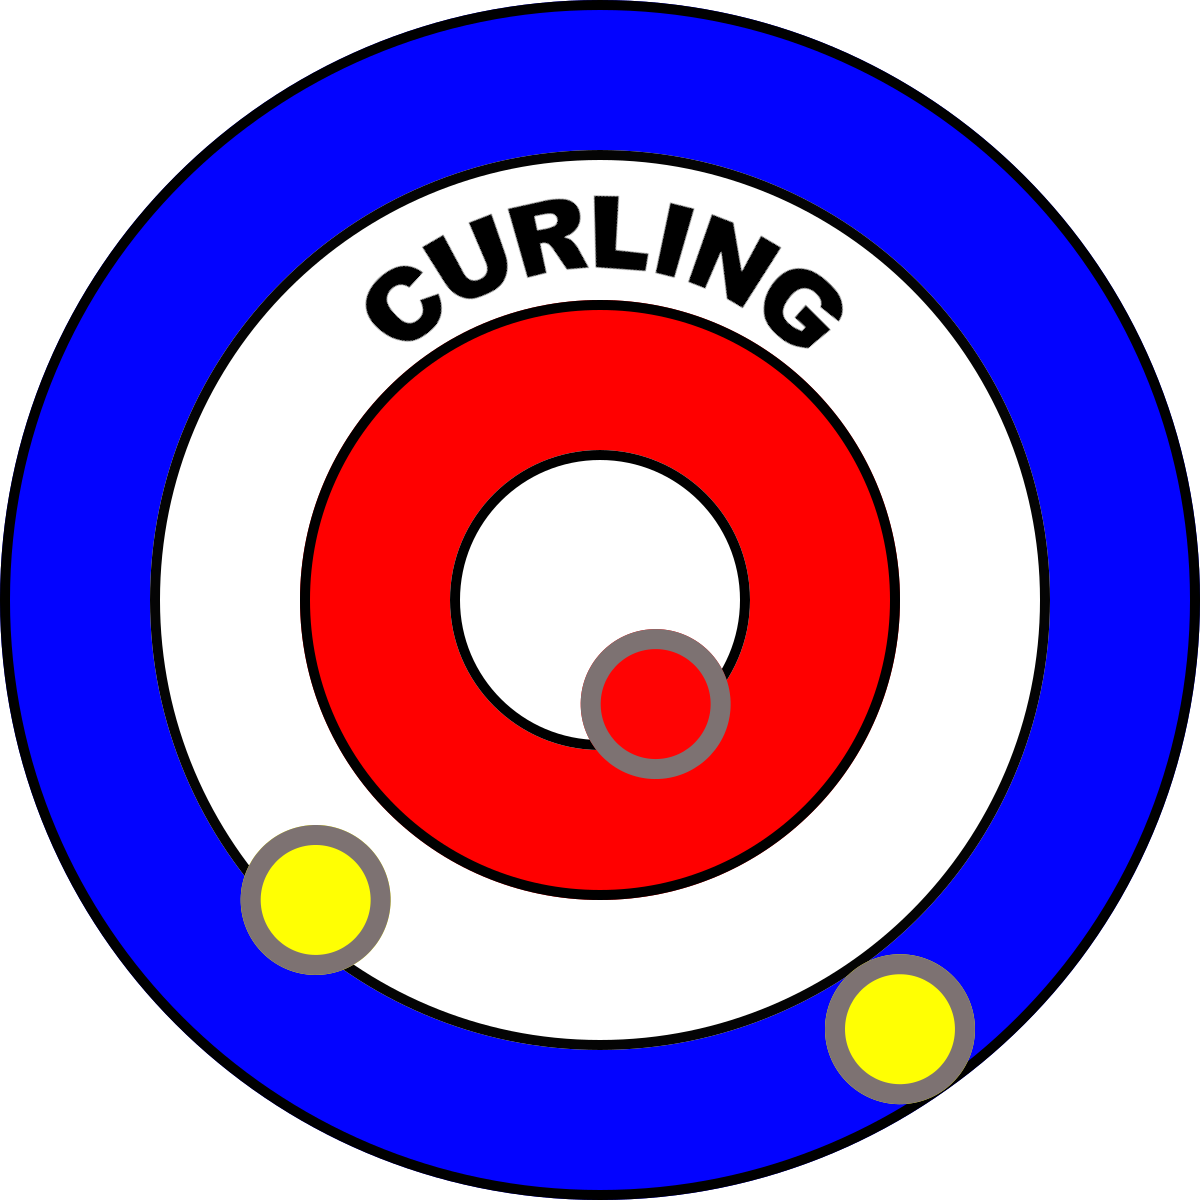
\includegraphics[width=\textwidth]{media/curling_logo}
    \begin{center}
        Modul 152 \\
        Multimediainhalte in einen Webauftritt integrieren\\
        E-Portfolio
    \end{center}}
\author{Tobias Hilfiker}
\date{\today}

% Document
\begin{document}

    %Kapitel Frontpage
    \begin{titlingpage}
        \maketitle
    \end{titlingpage}
    \pagebreak

    %Kapitel Table of contents
    \tableofcontents
    \pagebreak

    %Kapitel 1 - Einleitung
    \section{Einleitung}
    Im vorgehenden Storyboard habe ich die Umsetzung der Webseite beschrieben, welche ich im Rahmen dieses Projektes umsetzen darf. Während des
    E-Portfolios sollten folgende Unteraufgaben erfüllt werden:

    \begin{itemize}
        \item Responsive-Webseite anhand des Mockups im Storyboard umsetzen
        \item Video über das gewählte Thema filmen und schneiden
        \item Minimum drei Bilder machen und diese mit einer Bildmanipulation versehen
        \item Multimediaelemente aus den letzten zwei Punkten in die Webseite einbinden
        \item Prozess der oben genannten Punkten in dieser Dokumentation dokumentieren
    \end{itemize}
    \\
    \\
    Der gesamte Code + \LaTeX\xspace Dokumentation sind auf Github unter folgendem Link zu finden:\\
    \url{https://github.com/Ramspopoo/Modul_152}\\
    Das Storyboard wie auch das E-Portfolio habe ich zusätzlich als Release hinzugefügt, damit keine Daten verändert werden können.
    Um sich die Webseite im Internet anzusehen, wurde sie unter folgender URL veröffentlicht:\\
    \url{http://webseiten.informatik.sg/2022/ina4a/gruppe4/}
    \pagebreak

    %Kapitel 2 - Webseite
    \section{Webseite}
    Nachfolgend werde ich erläutern, wie ich die Webseite umgesetzt habe. Anfangs werde ich zudem die von mir verwendeten Technologien aufzeigen.
    Am Schluss werde ich über den Arbeitsprozess der Webseitenerstellung reflektieren.

    %Kapitel 2.1 - Eingesetzte Technologien
    \subsection{Eingesetzte Technologien}
    Um die Webseite zu erstellen habe ich diverse Technologien eingesetzt. Diese möchte ich in den folgenden zwei Abschnitten erläutern.

    %Kapitel 2.1.1 - Basics
    \subsubsection{Basics}
    Um Skizzen auf der Webseite zu erstellen habe ich Adobe Xd verwendet. Dies aus zwei Gründen:
    \begin{enumerate}
        \item Ich kann die Assets als SVG exportieren. Diese werden dann nicht allzu gross und können optimal skaliert werden.
        \item Ich habe bereits das Mockup mit Xd gemacht, daher hatte ich bereits Beispiele darin gezeichnet, welche ich wiederverwenden konnte.
    \end{enumerate}
    \\
    Da ich nicht oft in der Webentwicklung arbeite, hat mir Timo Tailwindcss als Framework fürs Styling empfohlen. Dadurch kann ich vereinfachte
    und vorgefertigte CSS-Klassen verwenden. Zudem hat es bereits eingebaute Media-Queries, was es einfacher macht, die Webseite responsive
    zu gestalten.
    %TODO cloudniary!!!!!

    %Kapitel 2.1.2 - Dev-Server und Plugins
    \subsubsection{Dev-Server und Plugins}
    Um bei mir lokal zu entwickeln, Plugins einzubinden und die Webseite zu compilen habe ich den Node Package Manager (NPM) verwendet.
    Zudem hat Timo mir \"Vite\" als Entwicklungsserver empfohlen, dieser recompilt die Seite automatisch nach jedem speichern des Files.
    Dabei zeichnet er sich dadurch aus, dass er diesen Reload sehr schnell ausführt.\\
    Um sogesehen Komponenten zu erstellen, habe ich ein Handlebar-Plugin für Vite verwendet. Damit kann ich einzelne kleine Files erstellen,
    welche dann eine Komponente darstellen. In diese Komponente kann ich dann Variabeln hineingeben, so kann ich in der Komponente auch sehr
    einfach z.B. den Text mittels Variable von aussen ändern und reduziere den benötigten Code.

    %Kapitel 2.2 - Umsetzung Webseite
    \subsection{Umsetzung Webseite}
    Anfangs war ich etwas verloren in der Umsetzung. Da ich wenig mit Webentwicklung zu tun hatte, wusste ich nicht recht wo ich anfangen sollte.
    Aber mit der Zeit kam ich gut in den Flow, und lernte auch immer mehr Tricks mit CSS und Tailwind kennen. Während der Umsetzung wurde die Zeit
    aber auch schnell knapp, wodurch ich einige Abweichungen zum Mockup machen musste. Diese habe ich nachfolgend dokumentiert.\\
    Ansonsten ging die Umsetzung recht gut vonstatten. Ich habe mir, wenn benötigt, Hilfe von Timo geholt, da er sich in der Webentwicklung wie auch
    mit Tailwind auskennt.

    %Kapitel 2.3 - Abweichungen Mockup
    \subsection{Abweichungen zum Mockup}
    Ich musste aufgrund von knapper Zeit und fehlendem Bild/Videomaterial einige Abweichungen zum Mockup machen. Diese möchte ich hier genauer erläutern.

    %Kapitel 2.3.1 - Seite "How To Play" nicht umgesetzt
    \subsubsection{Seite \"How to Play\" nicht umgesetzt}
    Aufgrund von fehlendem Bildmaterial und auch fehlender Zeit um eine Alternative zu suchen / erstellen, habe ich die Seite \"How to Play" nicht umgesetzt.
    Darauf sollte eigentlich beschrieben sein, wie ein Anfänger mit Curling beginnen soll. Im Nachhinein würde ich mir weniger einzelne Seiten vornehmen, und
    mir dann auch bereits beim Mockup-Zeichnen genauer Gedanken machen, wie ich die Seite später umsetzen werde.

    %Kapitel 2.3.2 - Seite "Beispiele" umbenannt
    \subsubsection{Seite \"Beispiele\" umbenannt}
    Während des Prozesses habe ich gemerkt, dass der Titel \"Beispiele\" für die Seite mit allen Bildern und Videos nicht sehr passend ist. Daher habe ich
    diese umbenannt auf den Namen \"Impressionen\". Dies passt viel besser zum Inhalt.

    %Kapitel 2.3.3 - Seiten mit Grid statt Banner
    \subsubsection{Seiten mit Grid statt Banner}
    Während der Umsetzung habe ich gemerkt, dass ein Banner mit überlappenden Elementen, wie ich es auf vielen Seiten des Mockups hatte, sehr
    schwierig umzusetzen ist. Es ist dann aber noch schwerer, dieses Banner responsive zu machen. Daher habe ich mich dazu entschieden,
    diese Elemente mit CSS Grid anzuordnen. So habe ich auch ein behandeltes Thema vom Unterricht in die Webseite eingebunden.

    %Kapitel 2.3.4 - Mobile Home-Page etwas anders gestylt
    \subsubsection{Mobile Home-Page etwas anders gestylt}
    Auf Mobile habe ich, statt die Navigationselemente im Banner über- / nebeneinander anzuordnen, diese untereinander angeordnet. Da es, aufgrund
    der gestrichenen \"How to Play\" Seite nur noch drei Seiten waren hätte es über- / nebeneinander schlecht ausgesehen, und so ist es auch
    einfacher für mich die Seite responsive zu machen, da ich nur den flex drehen muss.

    %Kapitel 2.3.5 - Logo und Navigation getauscht
    \subsubsection{Logo und Navigation getauscht}
    Um auf Mobile gleich auszusehen bzw. die gleiche Ausrichtung zu haben, habe ich die Position von Logo und Menü-Button im Vergleich zum Mockup
    getauscht. So ist nun das Menü (wie auf Desktop auch) auf der rechten Seite, und das Logo (wie auf Desktop) auf der linken Seite.

    %Kapitel 2.4 - Reflexion Webseite
    \subsection{Reflexion Webseite}
    Schlussendlich kann man sagen, dass ich ohne Hilfe von Timo und Tailwind die Webseite nie so gut hinbekommen hätte. Tailwind hat mir
    beim Styling und Responsive-Designen extrem viel Arbeit abgenommen, wofür ich sehr dankbar bin. Wie bereits gesagt hatte ich anfangs etwas
    Mühe, in den Aufbau und die Entwicklung der Webseite hineinzufinden. Zudem musste ich mich mit Tailwind zuerst zurechtfinden. Ich war zudem
    eine Woche krank, was dazu geführt hat, dass am Schluss alles schneller gehen musste, als ich mir das eigentlich gewünscht habe. Hätte ich noch
    eine Woche mehr Zeit, könnte ich einige vorher dokumentierte Abweichungen noch ausmerzen und die Webseite gesamt schöner machen.\\
    Während der Entwicklung der Webseite habe ich viel Neues über Webdesign gelernt und auch sehr vieles verstanden, was ich vorher einfach
    immer angewendet habe, aber nicht richtig wusste was wirklich dahinter steckt. So möchte ich mich in nächster Zeit mehr mit Webentwicklung
    befassen und auch Tailwind noch genauer anschauen, als ich das hier im Rahmen des E-Portfolios gemacht habe.

    %Kapitel 3 - Video
    \section{Video}
    In den folgenden Kapiteln werde ich erklären, wie ich das Video gefilmt habe und was die Schwierigkeiten dabei waren. Zudem werde ich
    erläutern, wie ich das Video geschnitten habe und über den ganzen Prozess reflektieren.

    %Kapitel 3.1 - Erstellung Video
    \subsection{Filmen Video}
    Mich stellte die von mir gesetzte Anforderung, dass ich gefilmt haben wollte, wie verschiedene Steine gespielt werden, vor eine Challenge.
    Denn am besten sieht es aus, wenn man Steine während dem Spiel von oben filmt. Wenn dies zum Beispiel an einer WM oder Olympia gemacht wird,
    werden über dem Spielfeld sogenannte Seilkameras aufgehängt. Diese sind an Seilen aufgehängt und hängen über dem Spielfeld. Mittels Motoren
    und Zugseilen können diese dann ferngesteuert werden und über das Spielfeld flitzen. Allerdings haben wir in der Curlinghalle in St. Gallen
    keine solchen Einrichtungen. Daher muss ich mir anders behelfen.\\
    Für mich war es am einfachsten, eine Drohne zu verwenden. Auch das war aber nicht sehr einfach. Denn in der Halle selbst habe ich aufgrund
    des Metalldachs keinen GPS-Empfang, was dazu führt, dass die Drohne nicht stabil an Ort und Stelle bleibt.
    Als Drohne habe ich eine DJI Mavic Air verwendet, welche eigentlich auch über ein sogenanntes \"FocusTrack\" Feature verfügt. Dieses erlaubt dem
    Pilot der Drohne, Objekte auszuwählen, welcher die Drohne automatisch folgt. Dieses habe ich aus folgenden zwei Gründen nicht verwendet
    / verwenden können:

    \begin{enumerate}
        \item Aufgrund des fehlenden GPS erlaubte mir die Drohne gar nicht, FocusTrack zu verwenden
        \item Es war mir zu riskant, die Drohne in der Halle automatisch fliegen zu lassen. Die Drohne durfte nämlich auf keinen Fall abstürzen,
        da sonst das Eis beschädigt werden könnte. Einfach unkontrolliert aufsteigen sollte sie aber auch nicht, da nach wenigen Metern
        die Hallendecke kommt.
    \end{enumerate}
    Daher blieb mir nichts anderes übrig, als die Drohne manuell hinter dem gespielten Stein hinterherzufliegen. Da dies recht anspruchsvoll ist
    und ich nicht gerade für mein Flugkönnen bekannt bin, habe ich einen Kollegen, welcher auch einige Jahre Curling gespielt hat, angefragt, ob er
    mir hilft zu filmen. Er fliegt in der Freizeit FPV-Drohnen (Drohne mit VR-Brille, mit welcher man die Perspektive der Drohne sieht) und kennt
    sich daher sehr gut mit dem Fliegen der Drohnen aus.\\
    Ich habe zudem geschaut, dass nicht zu viele Personen in der Halle sind, damit einerseits nicht zu viele zusätzliche Personen auf den Bildern
    sind, andererseits dass wir mit unseren Drohnenflügen nicht viele Personen in Gefahr bringen / stören.\\
    Abgesehen von den Anfangsschwierigkeiten mit dem GPS hatten wir während des Filmens keine Probleme.

    %Kapitel 3.2 - Schnitt des Videos
    \subsection{Schnitt des Videos}
    Ich war mir lange nicht sicher, wie ich das Video schneiden soll. Da ich mehrere einzelne Clips hatte, die ich einerseits kürzen und dann
    aneinanderreihen musste, brauchte ich ein Tool, welches dafür gut genug war. Bisher hatte ich Videos immer auf dem Handy geschnitten, was
    besonders mit den grossen Videodateien, welche die Drohne gespeichert hatte, sehr mühsam ist. Zudem hatte ich etwas Erfahrung mit Windows
    Movie Maker, allerdings gibt es diesen bereits seit Windows 8 nicht mehr. Da ich über die Schule ein Abonnement für die Adobe Creative Cloud
    habe, habe ich mich dann entschieden, ein Tool daraus zu nutzen. Da ich bereits mit Adobe Premiere Pro gearbeitet hatte und wusste, dass
    es sehr umfänglich und umständlich ist, wollte ich dieses Mal Adobe Premiere Rush ausprobieren.\\
    Premiere Rush ist sehr simpel ausgelegt, bietet mir aber alle Tools, die ich benötige. Zudem sind die Output-Files in einer sehr hohen
    Qualität, womit ich vor allem bei Movie Maker in der Vergangenheit Probleme hatte.\\
    Da Premiere Rush so einfach ausgelegt ist, war es auch keine grosse Sache das Video zu schneiden. Manchmal hatte der Laptop etwas Mühe,
    das Video immer flüssig abzuspielen. Ich kann aber nicht definitiv sagen, ob die CPU oder der RAM zu wenig Leistung hatte und so das Programm
    etwas blockiert hat.\\
    Ansonsten hat mich das Programm überzeugt, sprich ich werde es auch ein anderes Mal wieder verwenden, wenn ich ein Video schneiden muss.

    %Kapitel 3.3 - Reflexion Video
    \subsection{Reflexion Video}
    Das Video ist mir eigentlich sehr gut gelungen. Auch wenn ich einige Schwierigkeiten und Herausforderungen mit der Drohne meistern musste,
    hat dies sehr gut funktioniert. Allerdings wäre es schöner gewesen, wenn die Technik richtig funktioniert hätte und einige Bilder und vor allem
    Videos weniger verwackelt gewesen wären. Aber dafür, dass die Drohne manuell gesteuert wurde, sieht das Video sehr gut aus.\\
    Auch das Schneiden des Videos hat sehr gut geklappt, auch dort abgesehen von den technischen Schwierigkeiten die ich mit meinem Laptop hatte.
    Aber ich habe besonders beim Videodreh viel Neues gelernt und werde z.B. das nächste Mal, wenn ich ein Video schneiden muss wieder Adobe
    Premiere Rush verwenden.

    %Kapitel 4 - Bildmanipulationen
    \section{Bildmanipulationen}
    In den nachfolgenden drei Kapiteln werde ich die einzelnen Bildmanipulationen, die ich auf drei Bilder angewendet habe, genauer erläutern.
    Die Bilder habe ich ebenso wie das Video mit der Drohne aufgenommen.

    %Kapitel 4.1 - Bildmanipulation 1
    \subsection{Bildmanipulation 1}
    Die erste Bildmanipulation habe ich bereits im Storyboard benutzt. Ich habe ein Bild genommen, welches direkt das Haus mit Steinen darin
    zeigt, welches von gerade oben fotografiert wurde. Dieses Bild habe ich dann mit GIMP schwarz-Weiss eingefärbt, und nur die Steine farbig
    gemacht. So werden diese besonders hervorgehoben und stechen sehr heraus. Neben diesem Herausstechen verbessert es aber nicht wirklich was
    am Bild.\\
    Diese Bildmanipulation ist sehr einfach gelöst, aber meiner Meinung nach sieht sie in diesem Fall sehr gut aus.

    \noindent
    \begin{minipage}{0.5\textwidth}
        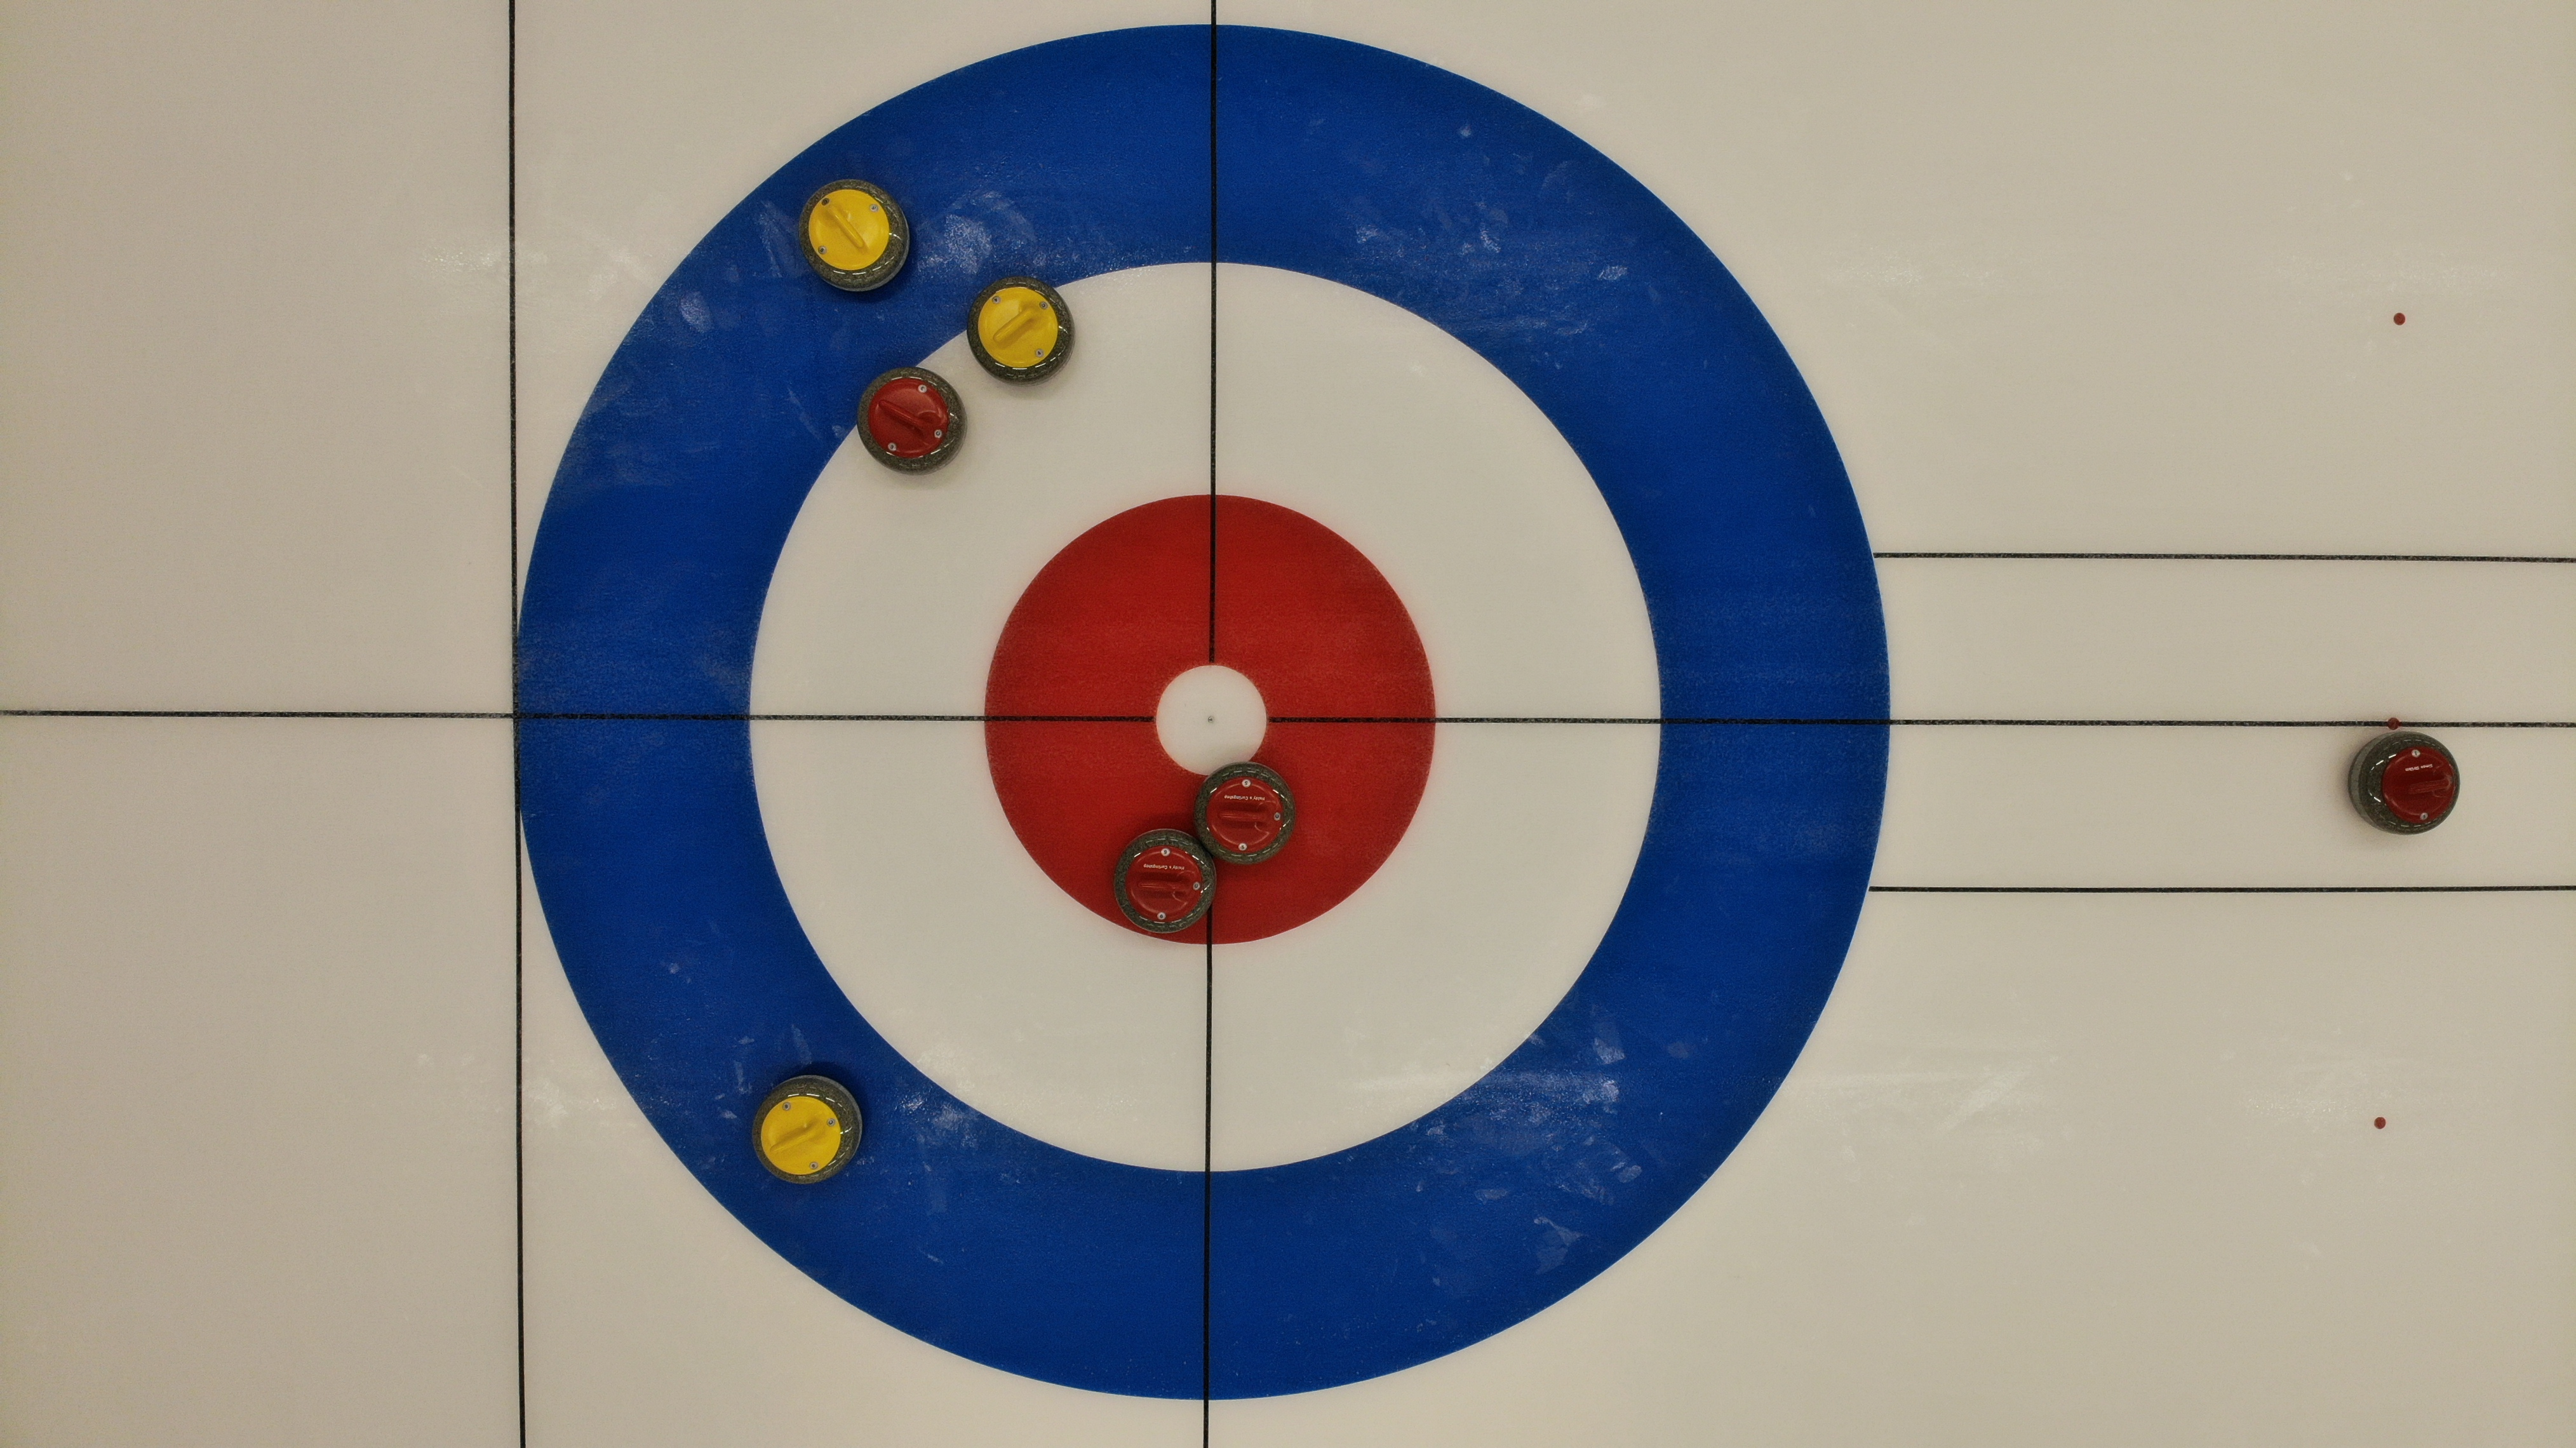
\includegraphics[width=\linewidth]{media/Black_White_Unedited}
    \end{minipage}
    \hfill
    \begin{minipage}[c]{0.5\textwidth}
        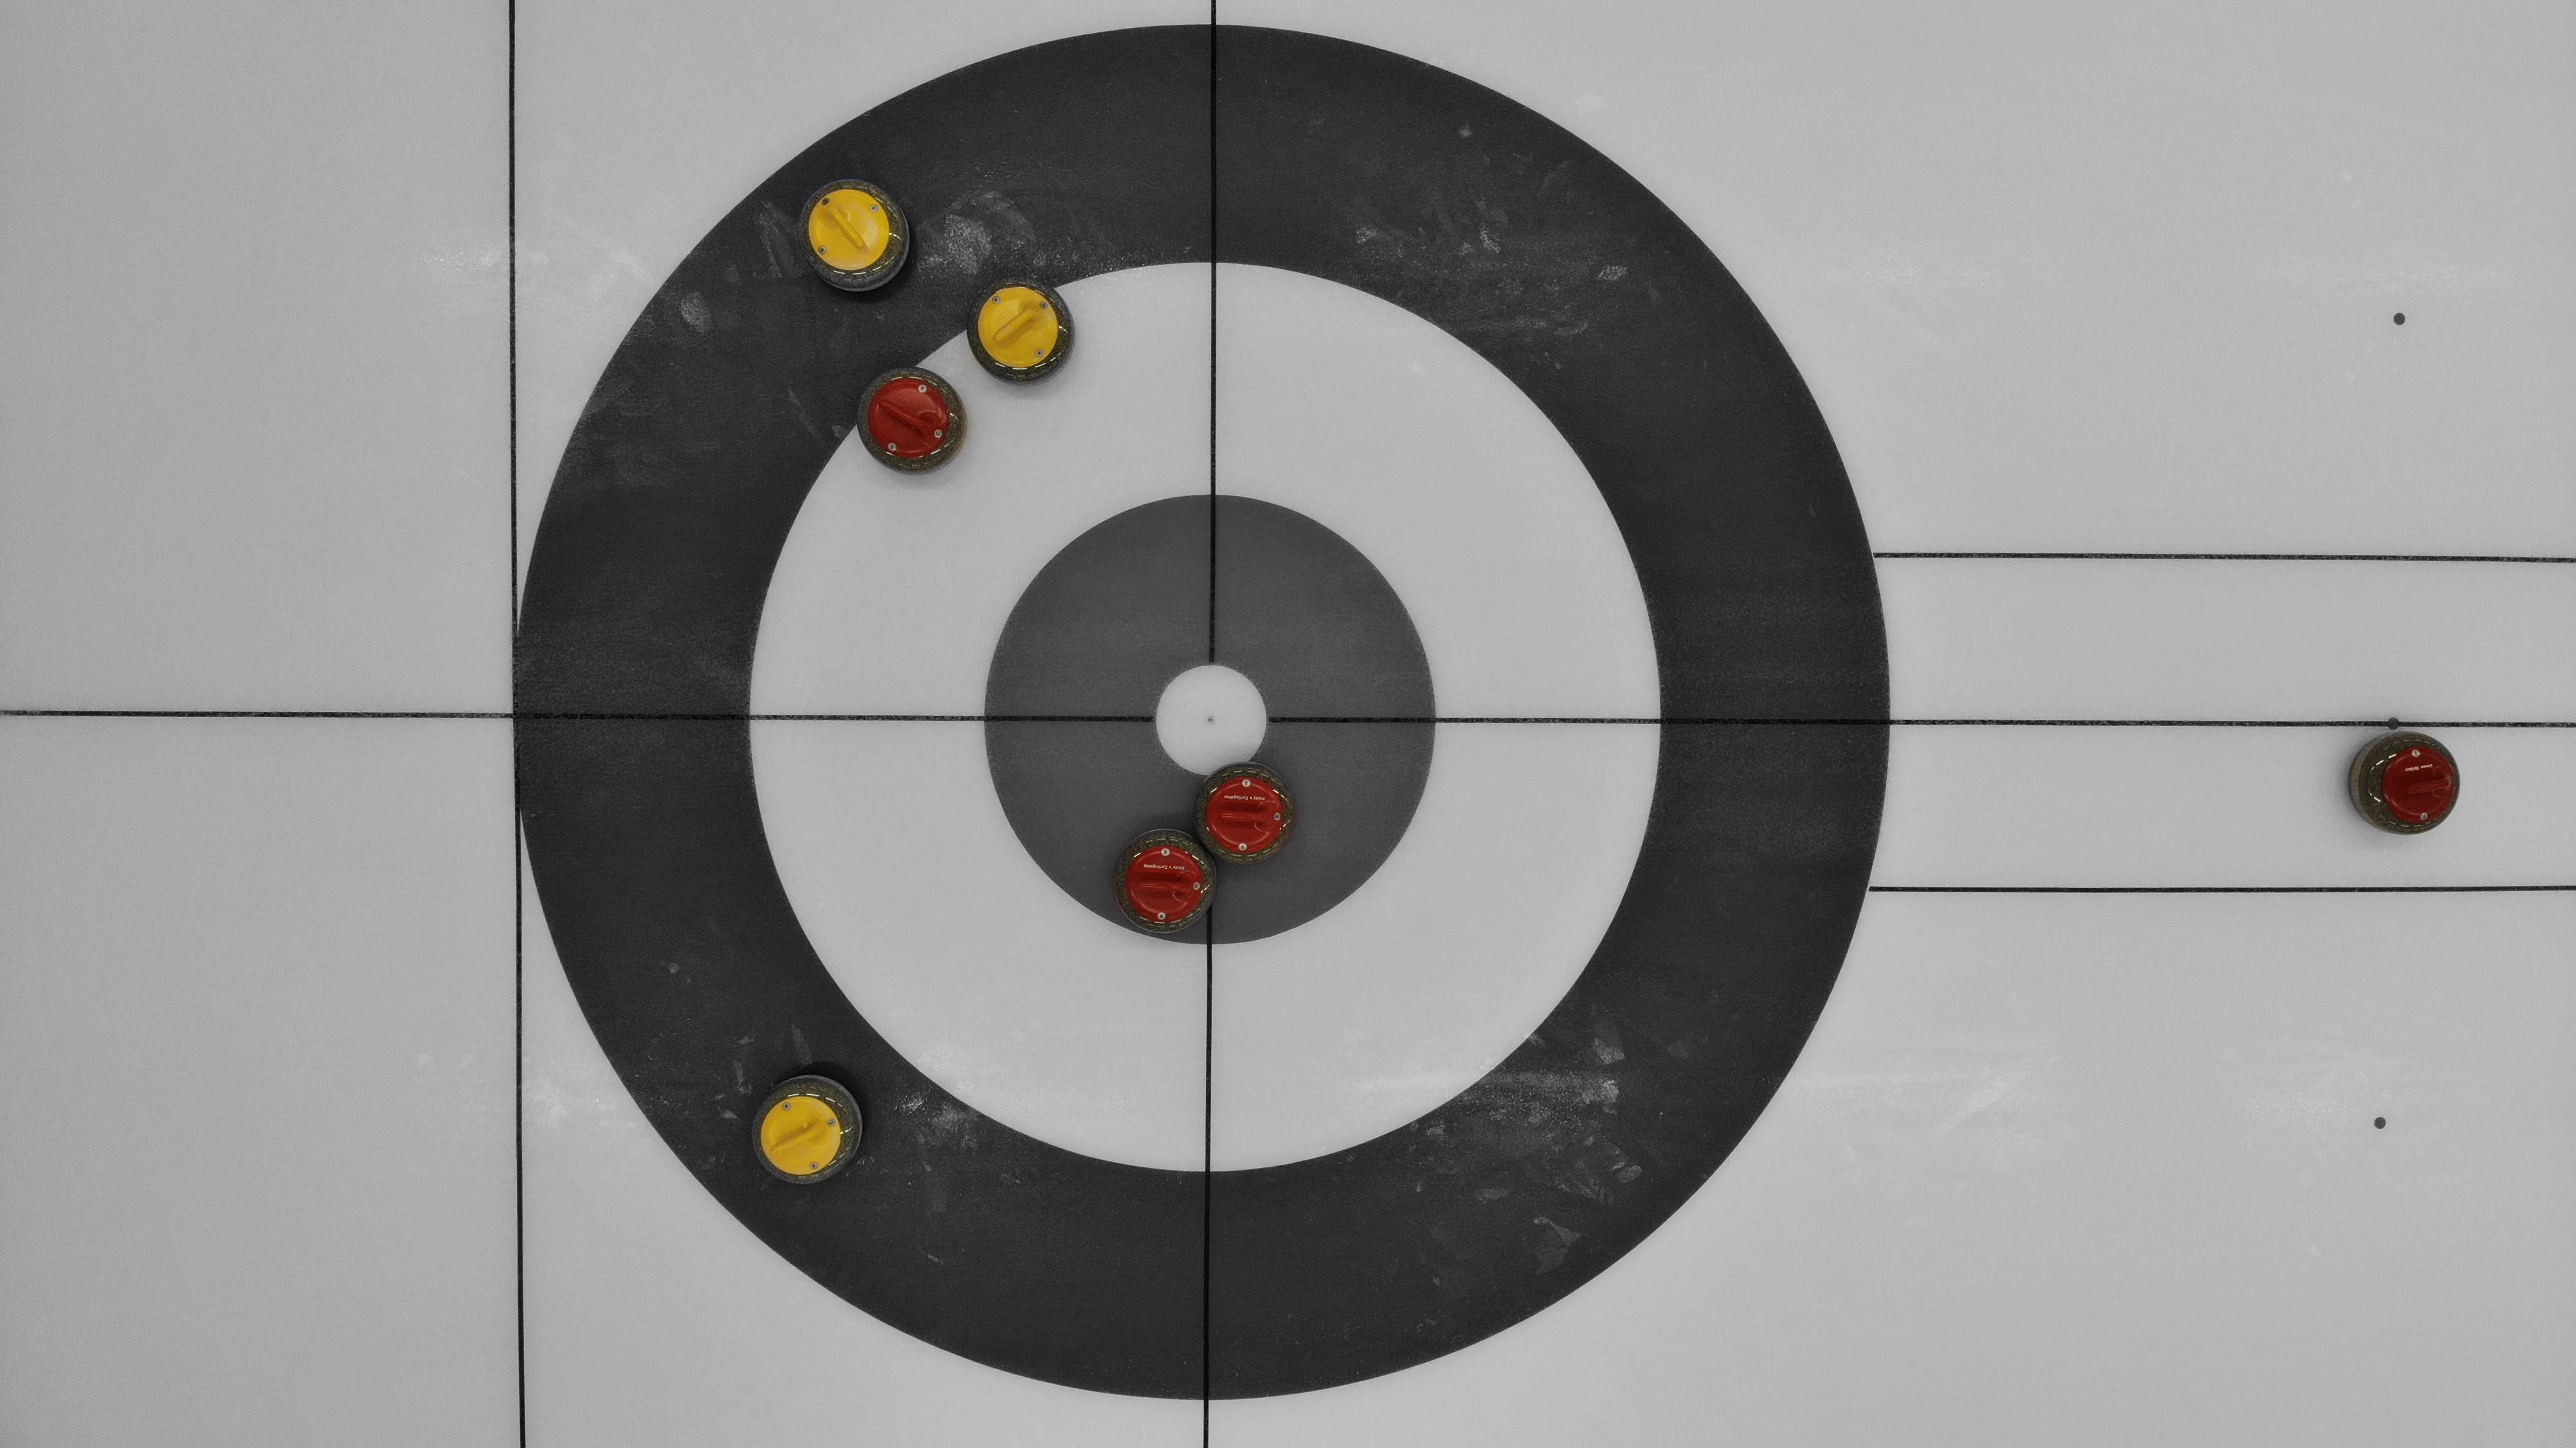
\includegraphics[width=\linewidth]{media/Black_White_Edited}
    \end{minipage}

    %Kapitel 4.2 - Bildmanipulation 2
    \subsection{Bildmanipulation 2}
    Als zweite Bildmanipulation habe ich auf dem Eis alle Werbungen entfernt. Das war eigentlich recht einfach, wenn das Eis nicht reflektieren
    würde. Dadurch hatte ich etwas probleme mit dunkleren und helleren Stellen im eis, die etwas schwieriger zu ersetzen waren. Wenn man aber
    nicht erwähnt, dass man Werbungen entfernt hat, würde man es nur beim sehr genauen Betrachten sehen. Eine zusätzliche Herausforderung war die
    Glasscheibe oben am Ende der Halle, welche die Werbungen noch reflektiert hat. Da es dahinter dunkel ist, kann man nicht genau sehen was
    eigentlich an diese Stelle gehört, und da an vielen Stellen die Werbung reflektiert hatte, war es etwas schwierig geeignete Stellen zum
    Ersetzen zu finden. Aber auch diese Bildmanipulation finde ich sehr passend zum Thema bzw. zum Bild. Denn die Halle wirkt ohne viele Farben
    auf dem Eis viel aufgeräumter.

    \noindent
    \begin{minipage}{0.5\textwidth}
        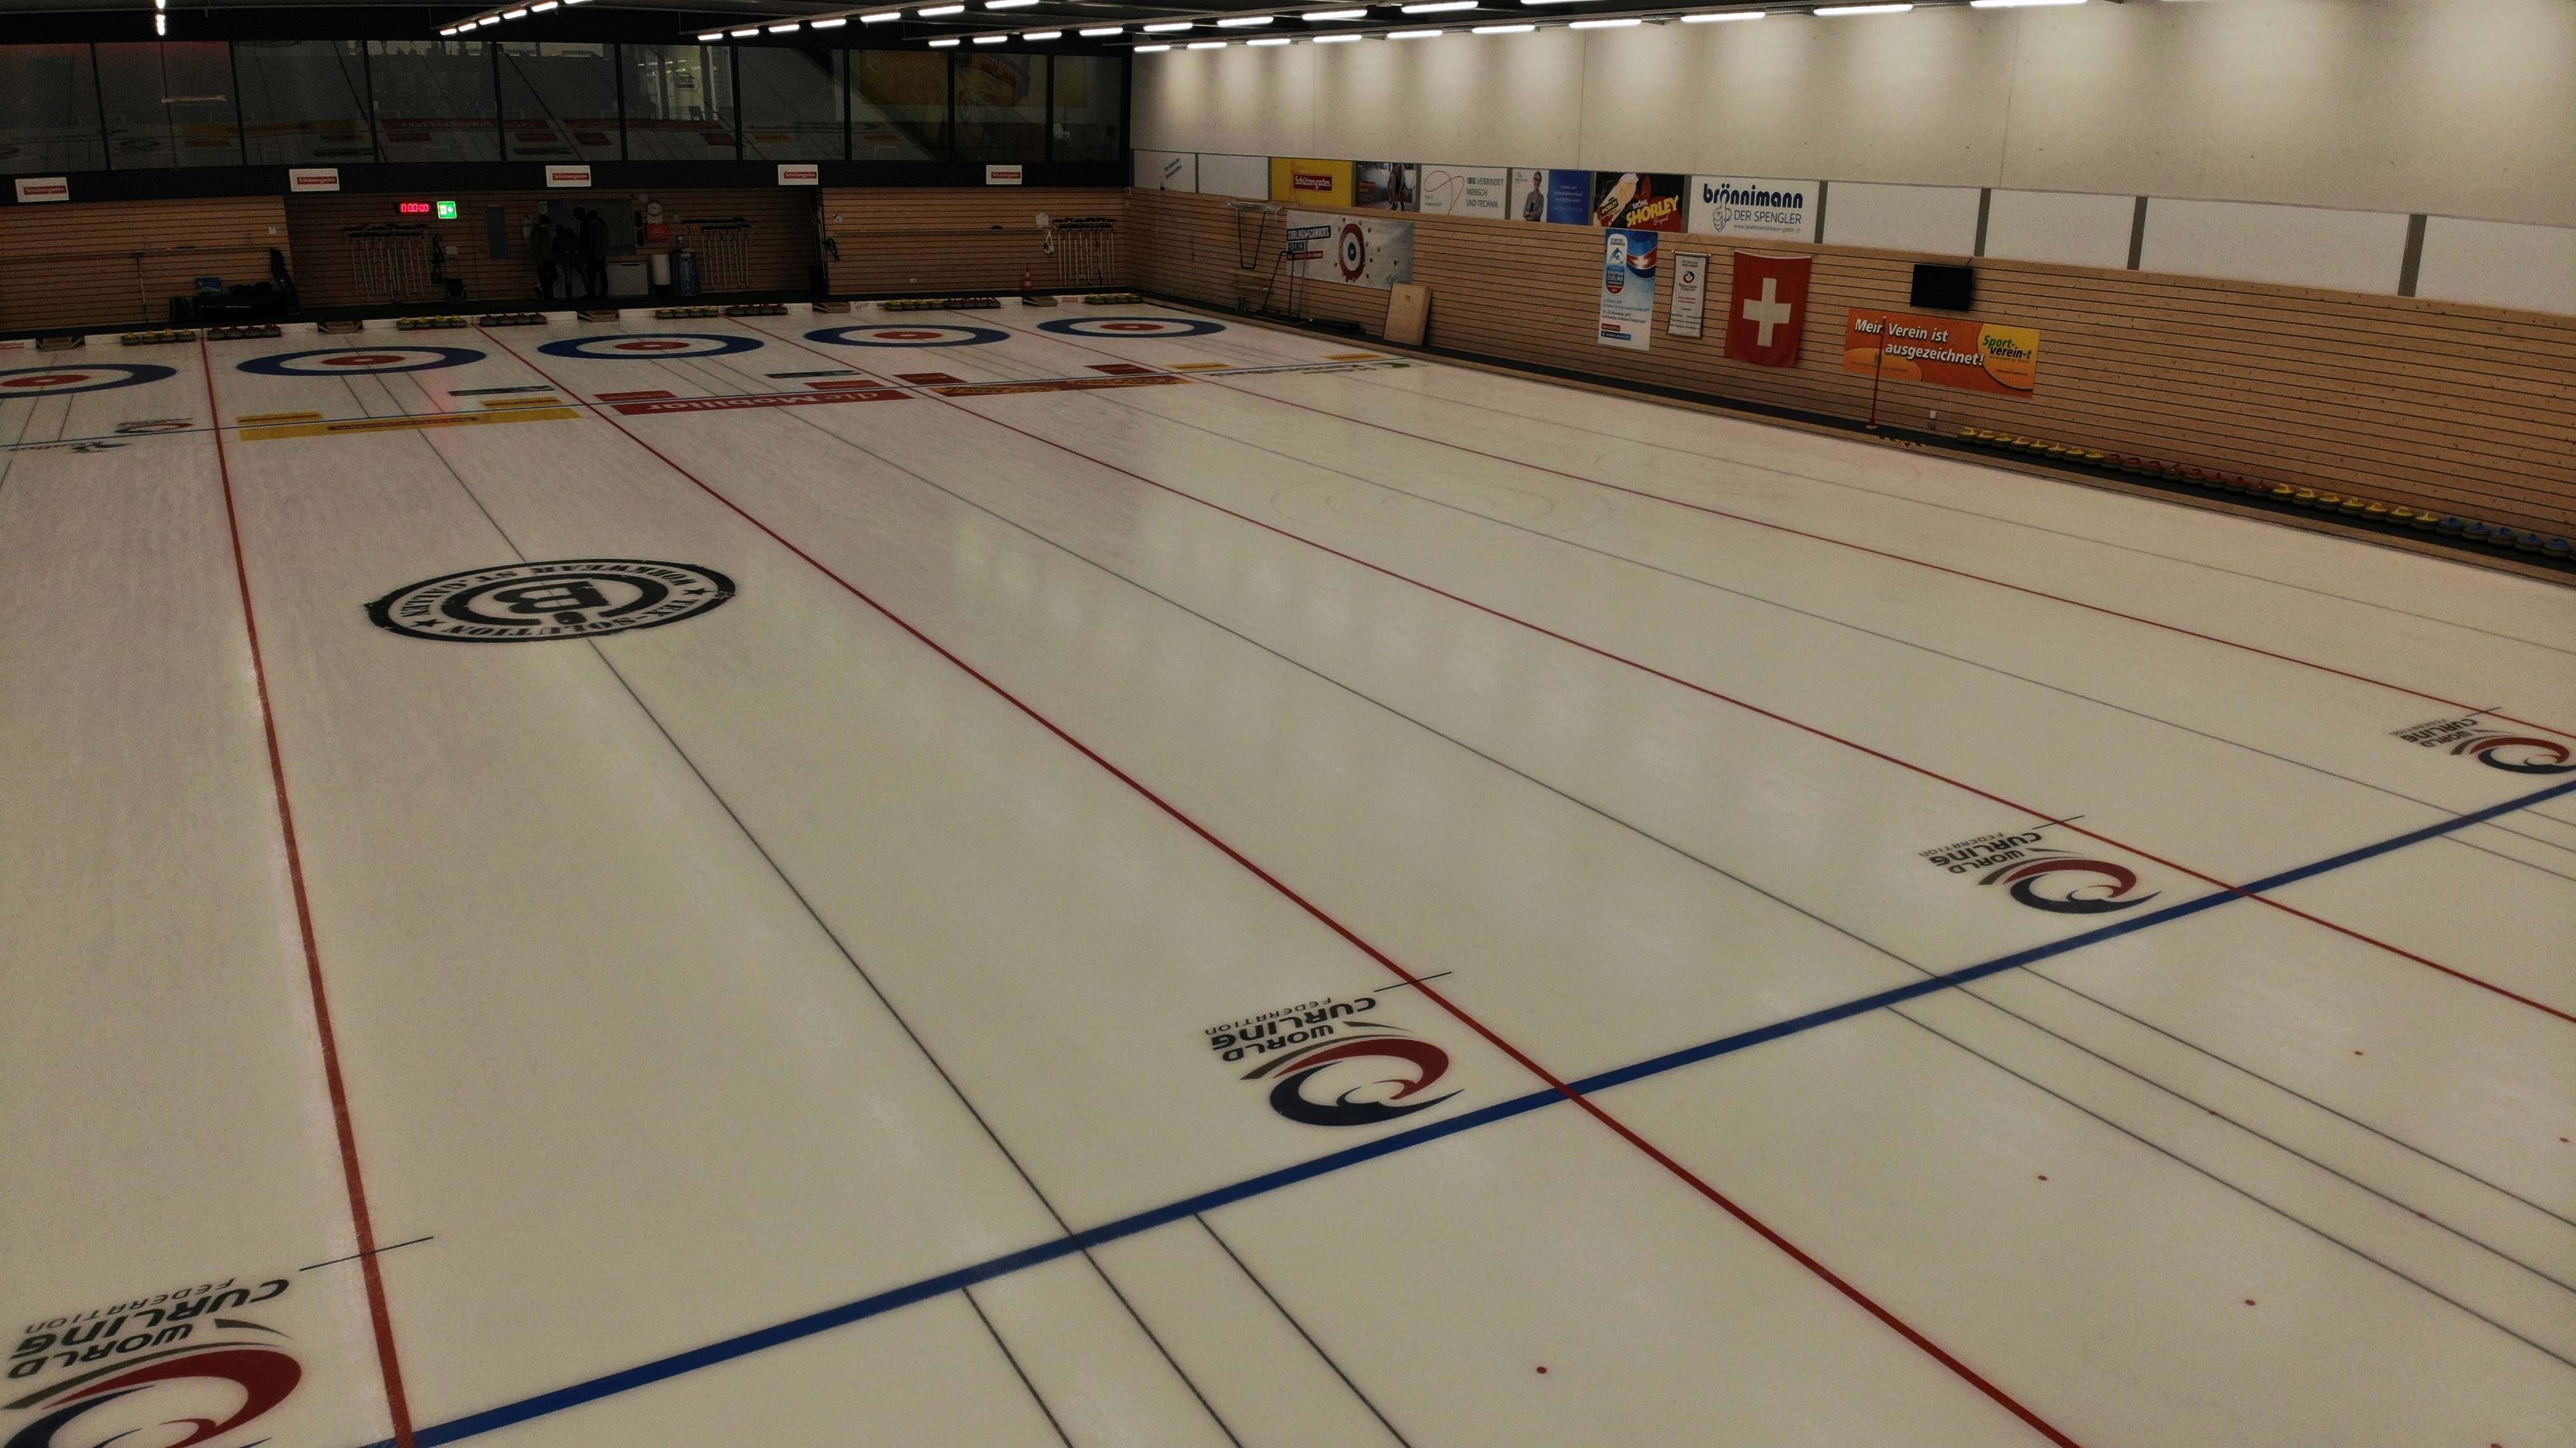
\includegraphics[width=\linewidth]{media/Advertisment_Unedited}
    \end{minipage}
    \hfill
    \begin{minipage}[c]{0.5\textwidth}
        \includegraphics[width=\linewidth]{media/Advertisment_Edited}
    \end{minipage}

    %Kapitel 4.3 - Bildmanipulation 3
    \subsection{Bildmanipulation 3}
    Als dritte Bildmanipulation wollte ich die Spiegelung im Eis durch das Licht reduzieren. Obwohl das sehr zum Bild passen würde, habe ich es
    leider nicht geschafft, den gewünschten Effekt zu erzielen. Ich habe es zwar geschafft die Spiegelug etwas zu reduzieren, ich hätte aber
    gerne länger experimentiert, bis sie noch mehr weg gewesen wäre. Ich habe hier mehrere verschiedene Möglichkeiten probiert, mit denen man
    in GIMP eigentlich solche Spiegelungen reduzieren können müsste. Allerdings haben alle bei mir nur so semi-gut funktioniert, dieses Bild
    ist noch am besten herausgekommen von allen versuchten Methoden.

    \noindent
    \begin{minipage}{0.5\textwidth}
        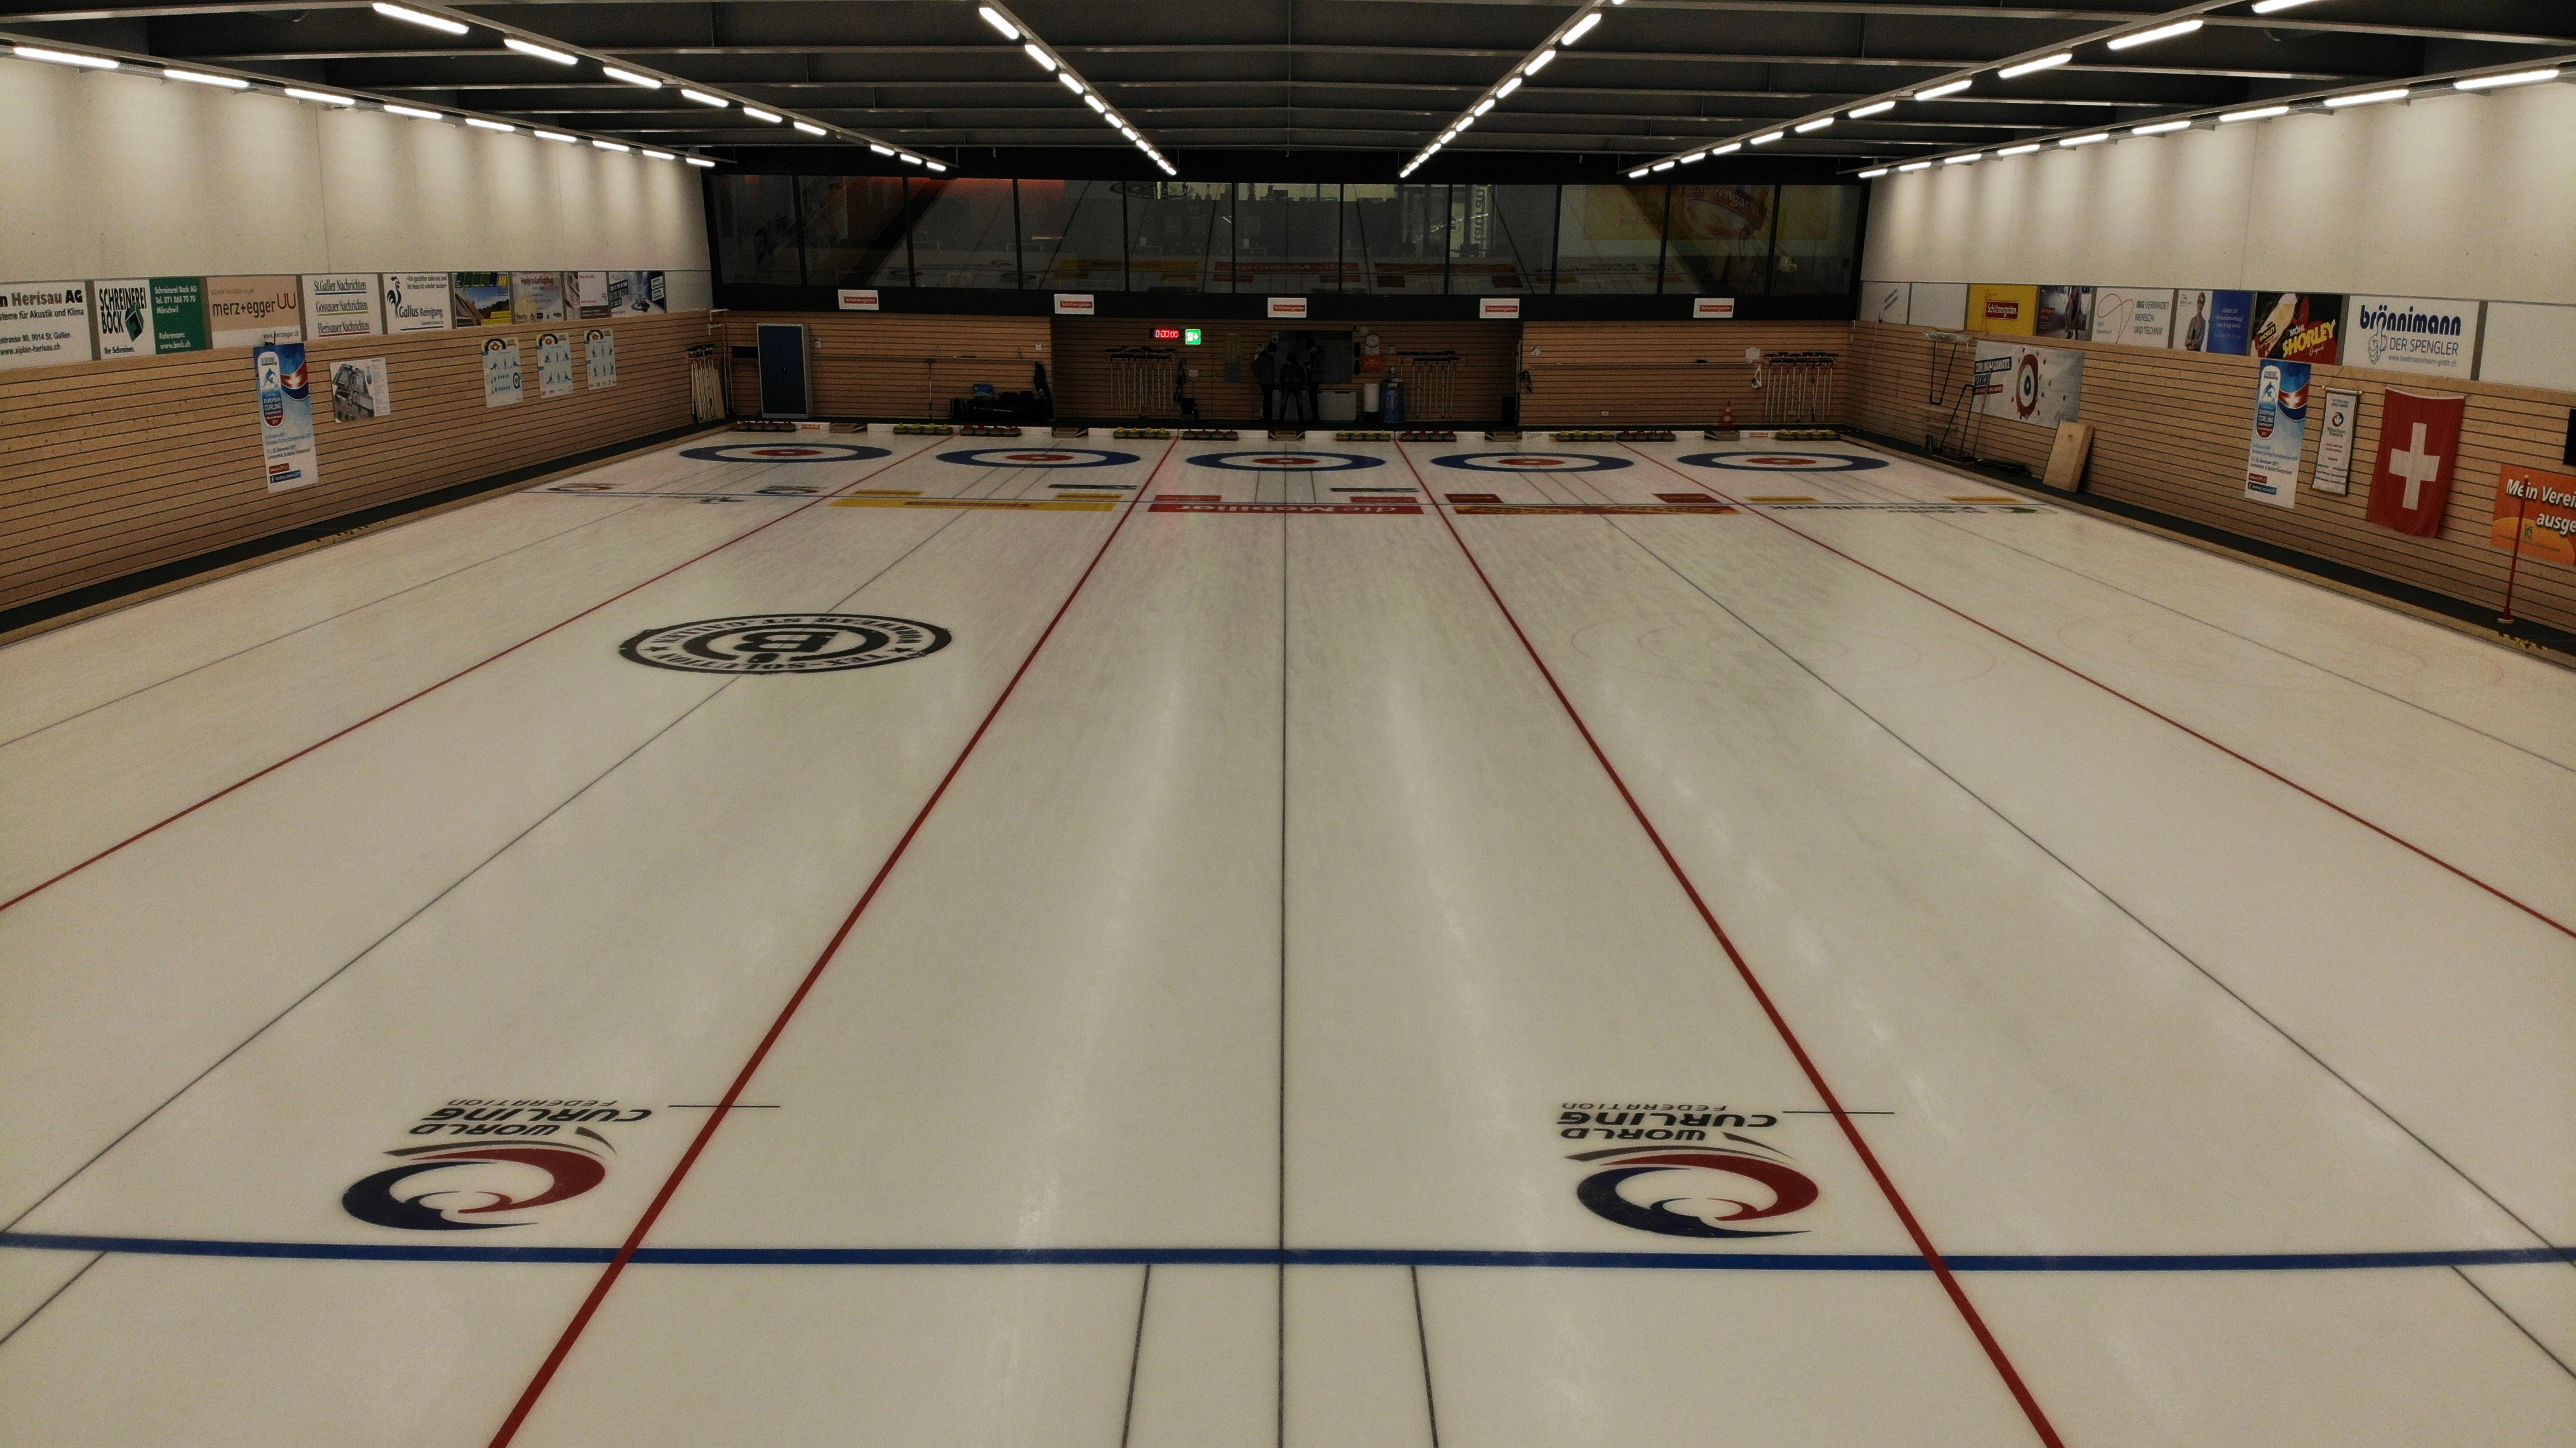
\includegraphics[width=\linewidth]{media/Glare_Unedited}
    \end{minipage}
    \hfill
    \begin{minipage}[c]{0.5\textwidth}
        \includegraphics[width=\linewidth]{media/Glare_Edited}
    \end{minipage}

    %Kapitel 4.4 - Reflexion Bildmanipulationen
    \subsection{Reflexion Bildmanipulationen}

    %Kapitel 5 - Fazit
    \section{Fazit}

\end{document}